\documentclass{scrarticle}

\usepackage[utf8]{inputenc}
\usepackage{xcolor}
\usepackage{bm}
\usepackage{amsmath}
\usepackage{amssymb}
\usepackage{graphicx}
\usepackage[outercaption]{sidecap}  
\usepackage{caption}
\usepackage{subcaption}
\usepackage{placeins}
\usepackage{url}
\usepackage{hyperref}
\usepackage{cleveref}

\usepackage{biblatex}
\addbibresource{references.bib}

\title{\Huge Dynamical Systems Theory in Machine Learning and	Data Science\\\huge - \\Final Project\\\vspace{1cm}\normalsize\texttt{\url{https://github.com/ZiqiuZhou/DST_final_project}}}
\author{Ziqiu Zhou\footnote{matriculation number: \textbf{3635588}. I need a grade, and I want to pick ex03, ex05, ex06, ex07, ex08, ex09 and ex10 for grading.}\\\small \href{mailto:fo249@stud.uni-heidelberg.de}{\texttt{fo249@stud.uni-heidelberg.de}} \and  Christoph Bender\footnote{matriculation number: \textbf{4012810}. I do not want a grade (only a pass and the 6 CP).}\\\small \href{mailto:Christoph.Bender@stud.uni-heidelberg.de}{\texttt{Christoph.Bender@stud.uni-heidelberg.de}}}



\begin{document}
	\maketitle
	
	\clearpage
	\documentclass{scrarticle}

\usepackage[utf8]{inputenc}
\usepackage{xcolor}
\usepackage{bm}
\usepackage{amsmath}
\usepackage{amssymb}
\usepackage{graphicx}
\usepackage{caption}
\usepackage{url}
\usepackage{hyperref}

\usepackage{biblatex}
\addbibresource{references.bib}

\title{DST - Final Project}
\author{Ziqiu Zhou (\textbf{\textcolor{red}{YOUR MATRIKELNUMBER}}), Christoph Bender (\textbf{4012810})}


\begin{document}
	\maketitle
	\clearpage
	\section{Summary LSTM \cite{Vlachas}}
	The invention of LSTM was motivated by the regularization of recurrent neural networks (RNNs). In addition to inputs $\bm{i}_t \in \mathbb{R}^{d_i}$, RNNs use also loops in order to include informations from previous hidden states $\bm{h}_{t'}$(where $t'<t$) in the calculation of the current state $\bm{h}_t \in \mathbb{R}^{d_h}$ at time $t$. The Elman network \cite{Elman} is for example defined by \footnote{see also \url{https://en.wikipedia.org/wiki/Recurrent_neural_network\#Elman_networks_and_Jordan_networks}}:
	\begin{figure}[h]
	\begin{minipage}[h][3cm][t]{7cm}
	\begin{align}
		\bm{h}_t&=\sigma_h(\bm{W}_{hi}\cdot\bm{i}_t+\bm{W}_{hh}\cdot\bm{h_{t-1}}+\bm{b}_h)\\
		\bm{o}_t&=\sigma_o(\bm{W}_{oh}\cdot\bm{h}_t+\bm{b}_o) \in \mathbb{R}^{d_o} \quad \footnotemark
	\end{align}
	\vfill
	\caption{Schematic Sketch of a RNN \cite{Vlachas}}
	\end{minipage}
	\begin{minipage}[h][3cm][c]{7.5cm}
		\centering
		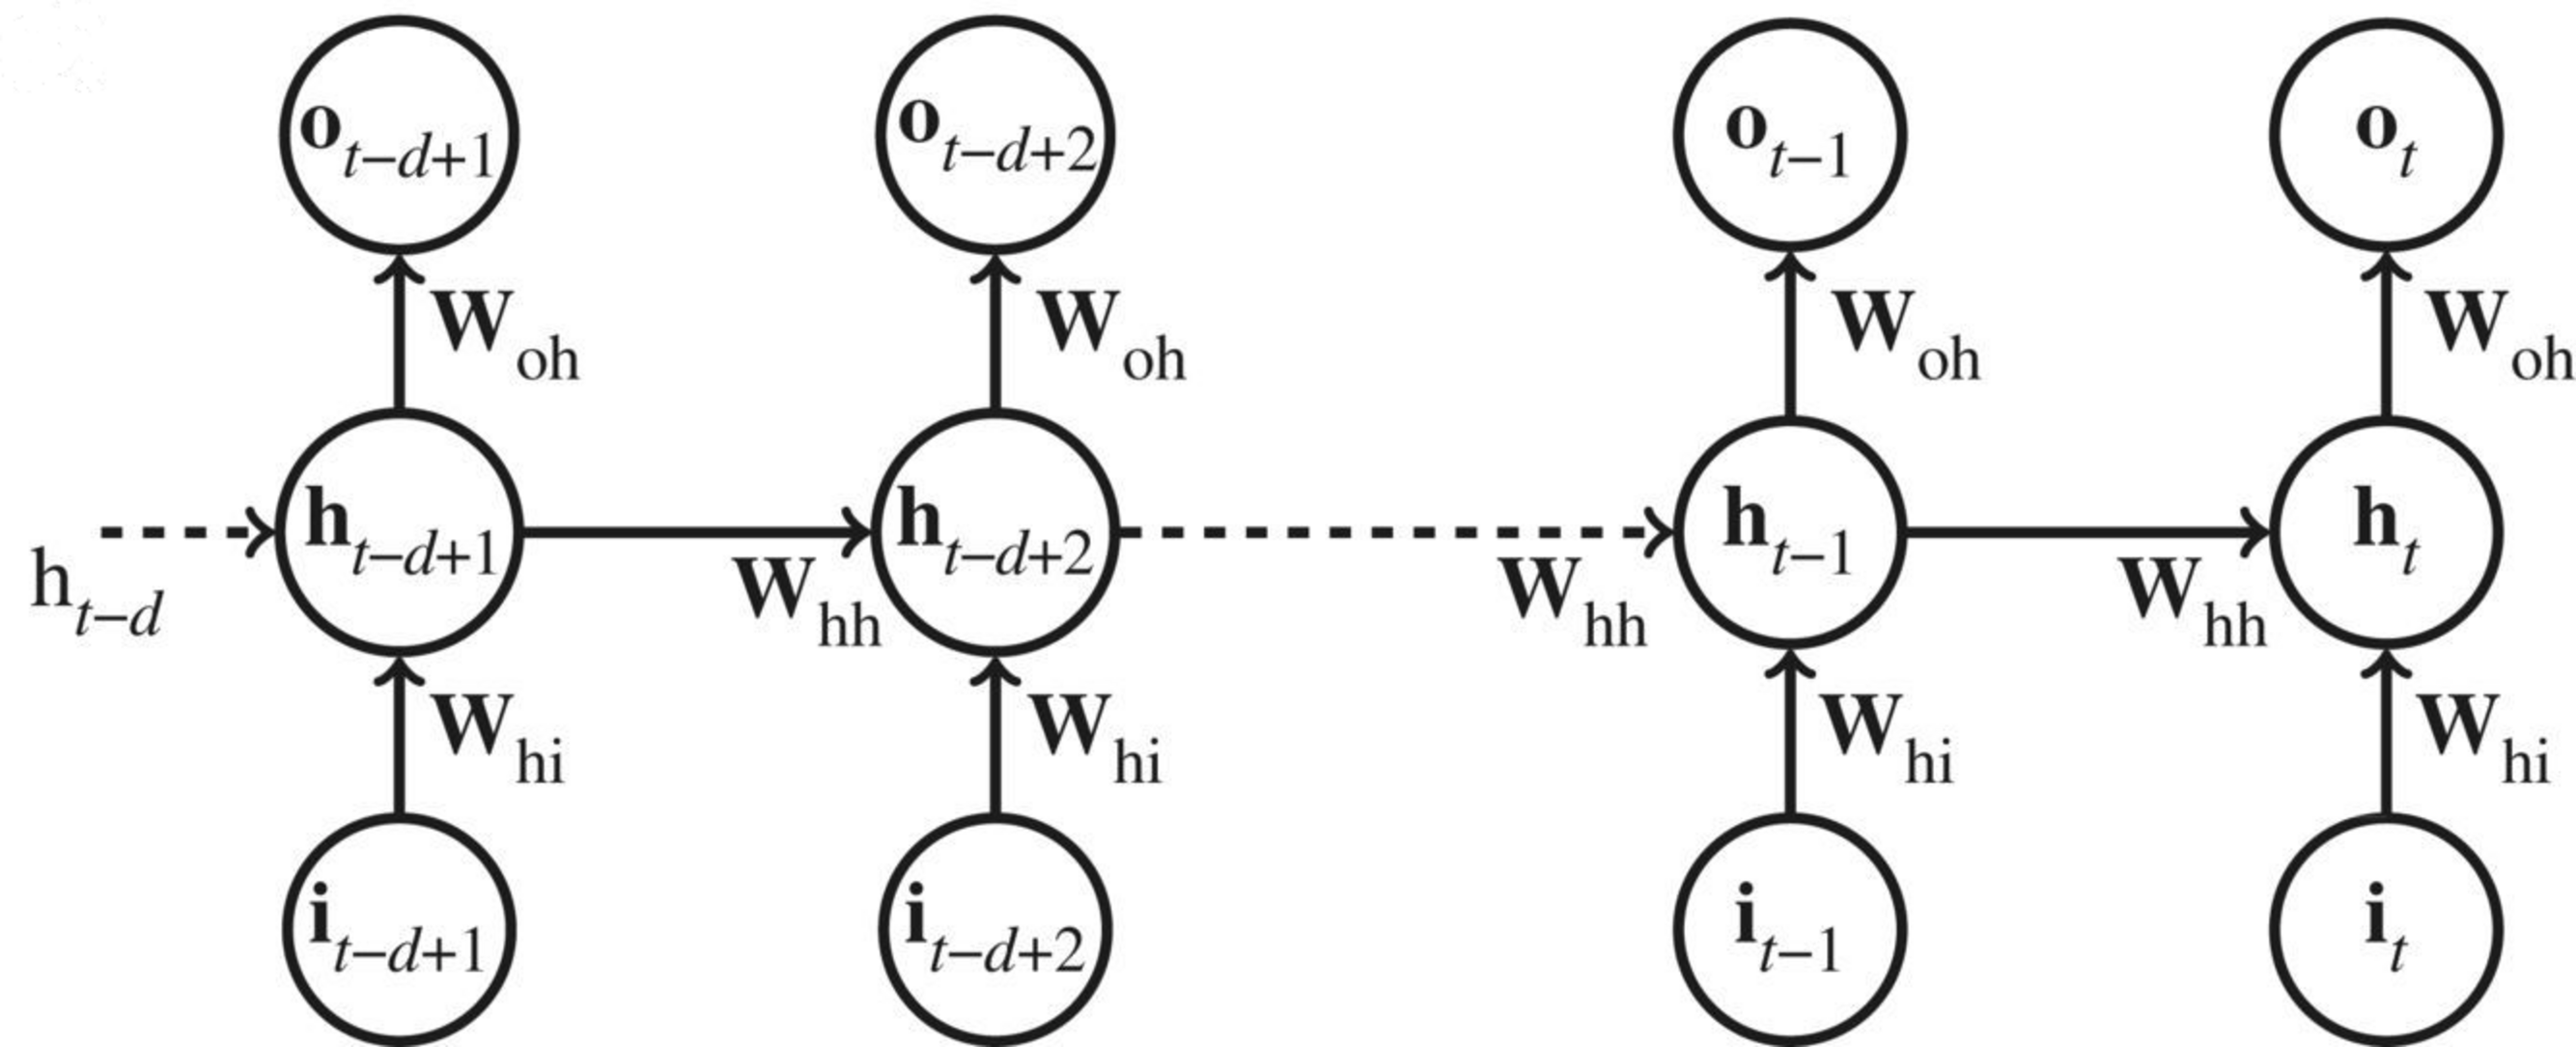
\includegraphics[width=7.3cm]{images/RNN_Vlachas_cropped.png}
	\end{minipage}
	\end{figure}
	\footnotetext{where $\sigma_\bullet$ are activation functions, $\bm{W}_{*\bullet}$ weight matrices and $\bm{b}_\bullet$ bias summands.}
	However RNNs struggle to recognize long-term dependencies and furthermore the gradient can vanish or explode, which also leads to problems. Because of this one uses gates. The corresponding model is called LSTM (Long Short-Term Memory). This is characterised by the following formula:
	\begin{equation}
	\begin{aligned}
		&\bm{g}^f = \sigma_f(\bm{W}_f\cdot[\bm{h}_{t-1}, \bm{i}_t]+\bm{b}_f)\\
		&\tilde{\bm{C}}_t = \text{tanh}(\bm{W}_C\cdot[\bm{h}_{t-1}, \bm{i}_t]+\bm{b}_C)\\
		&\bm{g}_t^o=\sigma_h(\bm{W}_h\cdot[\bm{h}_{t-1}, \bm{i}_t]+\bm{b}_h)
	\end{aligned}
	\quad
	\begin{aligned}
		&\bm{g}_t^i=\sigma_i(\bm{W}_i\cdot[\bm{h}_{t-1}, \bm{i}_t]+\bm{b}_i)\\
		&\bm{C}_t = \bm{g}_t^f\cdot\bm{C}_{t-1} +\bm{g}_t^i\cdot\tilde{\bm{C}}_t\\
		&\bm{h}_t = \bm{g}_t^o\cdot\text{tanh}(\bm{C}_t)
	\end{aligned}
	\end{equation}
	Whereby $\bm{g}_\bullet\in\mathbb{R}^{d_h\times(d_h+d_i)}$ represents the gate signal and $\bm{C}_t\in\mathbb{R}^{d_h}$ the so-called cell state, which is jointly with the hidden state referred as "LSTM states". To map the hidden state to the wanted output space one also uses an additional fully connected layer $\bm{W}_{oh}$:
	\begin{align}
		\bm{o}_t = \bm{W}_{oh}\cdot\bm{h}_t = f^w(\bm{z}_t, \bm{h}_{t-1}, \bm{C}_{t-1}) \approx F^w(\bm{z}_t, \bm{z}_{t-1}, \hdots, \bm{z}_{t-d+1}) \quad\footnotemark
	\end{align}
	\footnotetext{where in the following $\bm{z}_t$ is used as the input and describes the system time series.} 
	The so-called LSTM cell-function $f^w$ can be rewritten by iterative repition as $F^w$, where $w$ includes all trainable parameters. In the last step one uses the assumption that d-time steps are sufficient to compute the current output and thus $\bm{h}_{t-d},\bm{C}_{t-d}$ can be omitted.
	Goal of the LSTM is to predict the state derivative $\bm{\dot{z}}_t$ using a short time memory of the $d$ previous states $\bm{z}_{t:t-d+1}$. Therefore, the loss $\mathcal{L}$ shall be minimized by searching for the best parameters $w^*$:
	\begin{align}
	w^* = \arg\min_w\mathcal{L}(\{\bm{z}_{1:T},\bm{\dot{z}}_{1:T}\},w)=\arg\min_w\frac{1}{T-d+1}\sum_{t=d}^T||F^w(\bm{z}_{t:t-d+1})-\bm{\dot{z}}_t||^2
	\end{align}
	
	\section{Results}
	\textcolor{red}{What do you think about the idea to shortly present the results of task 3 here, i.e. saying the sigma and the cutoff frequency and maybe some training graphics ...}
	\subsection{Lorenz63}
	\subsection{Lorenz96}
	
	\printbibliography
\end{document}
	\FloatBarrier
	\section{Power spectrum metric}

The second task of the project was to implement the power-spectrum correlation (PSC). This features two hyperparameters: Namely
\begin{itemize}
	\item the smoothing factor $\sigma$, which is the width of the Gaussian kernel smoothing the spectrum
	\item and the cutoff, which excludes all frequencies above the given frequency threshold from the calculation of the power spectrum correlation.
\end{itemize}
The code snippets of \textit{psc.py} was added in \textit{global\_utils.py} and executed in \textit{rnn\_statefull.py}. Furthermore the plotting functions are added in the \textit{plotting\_utils.py} file.
In order to ensure that the model draws a random initial condition and then generates a time series of length T. We sampled random indices in the data generation and for each prediction the model takes one of these random integers during testing. And starts to predict the time series starting at the chosen starting point of the whole test series.

To illustrate the LSTM model and also to make sure whether the LSTM model is working, we first apply the model on a very simple sinosoidal dataset before applying it on the Lorenz datasets (see \cref{sec3}). For this we generate a time series consisting of 100000 points with time step size $\Delta t=0.5$ by computing:
\begin{align}
	z_t = A\cdot\sin(2\pi ft+\phi_0)+c
\end{align}
The chosen parameters are:
\begin{itemize}
	\setlength\itemsep{0.1em}
	\item amplitude $A = 2$
	\item frequency $f = 0.1$
	\item phase $\phi_0^{\text{train}}=0$, $\phi_0^{\text{test}}=0.5$
	\item offset $c=0.5$
\end{itemize}

Using the implemented LSTM Model of Vlachas et alium \cite{Vlachas}\footnote{\url{https://github.com/pvlachas/RNN-RC-Chaos}} one can train the LSTM model and test the LSTM model via the command line. The root mean squared error is chosen to be the loss, which is optimized during training. The loss decreases with increasing epochs for the training data and the validation data as well. This can be seen in \cref{2:loss}. Since validation loss is not increasing one can exclude the existence of overfitting.
\begin{figure}[h]
	\centering
	\begin{subfigure}[b]{0.45\textwidth}
		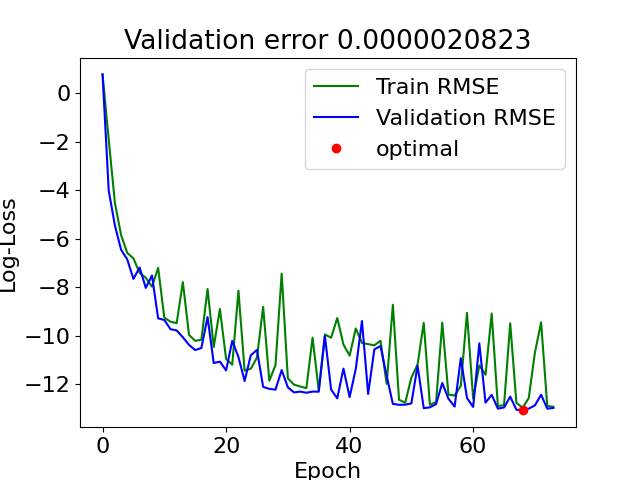
\includegraphics[width=\textwidth]{../Results/Test-Task02/Figures/RNN-lstm-RDIM_1-N_used_50000-NUM-LAY_1-SIZE-LAY_100-ACT_tanh-ISH_statefull-SL_8-PL_4-LR_0.001-DKP_1.0-ZKP_1.0-HSPL_300-IPL_200-NL_1-WID_0/Loss_total_log.png}
		\caption{Training and validation loss}
		\label{2:loss}
	\end{subfigure}
	\begin{subfigure}[b]{0.45\textwidth}
		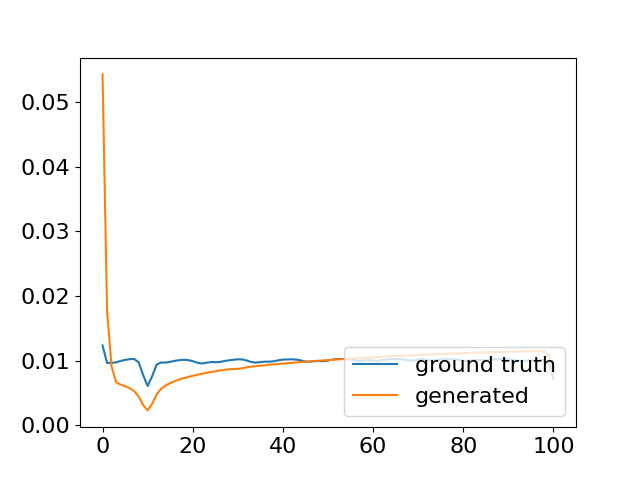
\includegraphics[width=\textwidth]{../Results/Test-Task02/Figures/RNN-lstm-RDIM_1-N_used_50000-NUM-LAY_1-SIZE-LAY_100-ACT_tanh-ISH_statefull-SL_8-PL_4-LR_0.001-DKP_1.0-ZKP_1.0-HSPL_300-IPL_200-NL_1-WID_0/spectrum_comparison_TEST.png}
		\caption{Power spectrum for test predictions}
		\label{2:spectrum}
	\end{subfigure}
\end{figure}

The plotted power spectrum shows a clear negative peak at 10, which corresponds to the chosen frequency of 0.1. %\textcolor{red}{\textbf{at ziqiu: do you know what the unit of the x-axis is?}}.
The power spectrum of the generated predictions show the same course of the curve as the ground truth, but appearently is shifted a bit. For the power spectrum plot we used a smoothing factor $\sigma=1$ and a frequency cutoff at 5000.

\FloatBarrier
Furthermore in \cref{2:predictions1} and \cref{2:predictions2} one can see the predictions of the LSTM of two test series with random chosen initial conditions and the corresponding errors. One can see that the LSTM can easily extract the sinosoidal behavior of the system and is able to fit to the data very well. However, one can see that the curves are a little bit off. Probably because the regressed frequency is not optimally. This explains why the error is increasing and accumulating the more the model predicts in the future.
\begin{figure}[h]
	\centering
	\begin{subfigure}[b]{0.45\textwidth}
		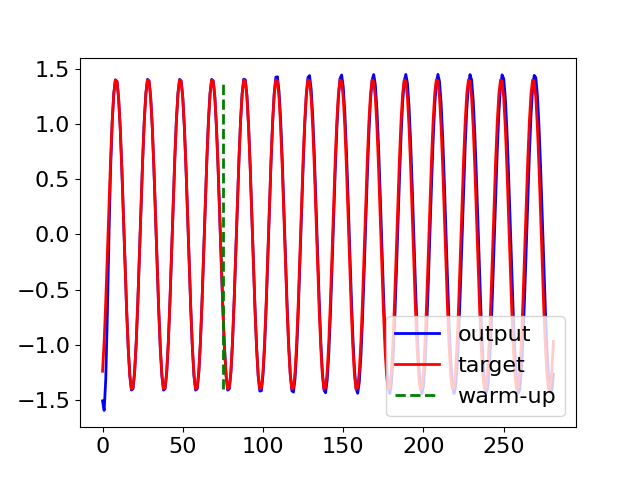
\includegraphics[width=\textwidth]{../Results/Test-Task02/Figures/RNN-lstm-RDIM_1-N_used_50000-NUM-LAY_1-SIZE-LAY_100-ACT_tanh-ISH_statefull-SL_8-PL_4-LR_0.001-DKP_1.0-ZKP_1.0-HSPL_300-IPL_200-NL_1-WID_0/prediction_augmend_TEST_70417.png}
		\caption{Prediction}
	\end{subfigure}
	\begin{subfigure}[b]{0.45\textwidth}
		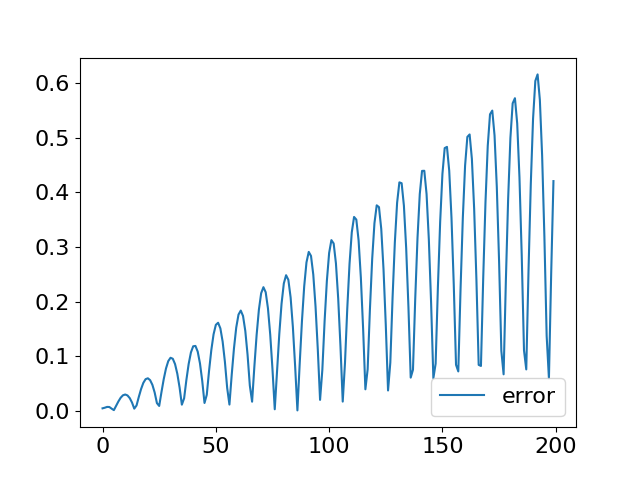
\includegraphics[width=\textwidth]{../Results/Test-Task02/Figures/RNN-lstm-RDIM_1-N_used_50000-NUM-LAY_1-SIZE-LAY_100-ACT_tanh-ISH_statefull-SL_8-PL_4-LR_0.001-DKP_1.0-ZKP_1.0-HSPL_300-IPL_200-NL_1-WID_0/prediction_TEST_70417_error.png}
		\caption{Error}
	\end{subfigure}
	\caption{Test results for random initial condition 70417}
	\label{2:predictions1}
\end{figure}
\begin{figure}[h]
	\centering
	\begin{subfigure}[b]{0.45\textwidth}
		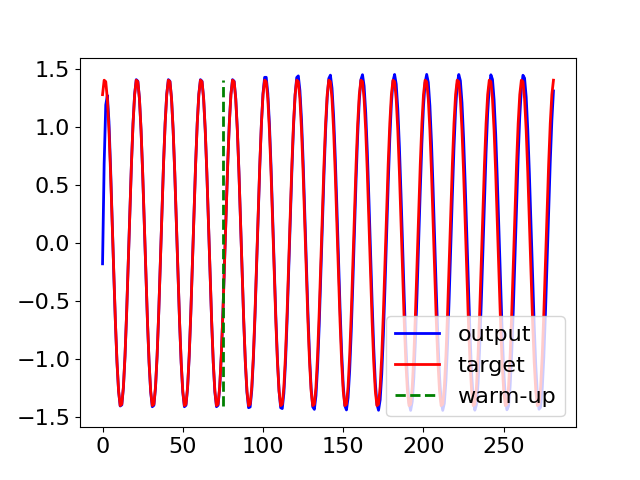
\includegraphics[width=\textwidth]{../Results/Test-Task02/Figures/RNN-lstm-RDIM_1-N_used_50000-NUM-LAY_1-SIZE-LAY_100-ACT_tanh-ISH_statefull-SL_8-PL_4-LR_0.001-DKP_1.0-ZKP_1.0-HSPL_300-IPL_200-NL_1-WID_0/prediction_augmend_TEST_98804.png}
		\caption{Prediction}
	\end{subfigure}
	\begin{subfigure}[b]{0.45\textwidth}
		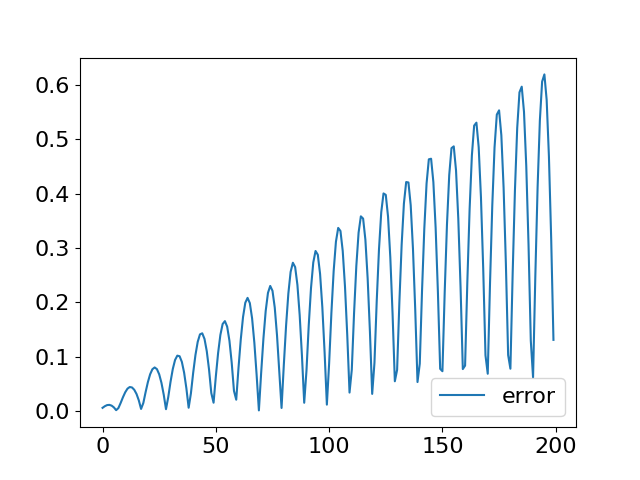
\includegraphics[width=\textwidth]{../Results/Test-Task02/Figures/RNN-lstm-RDIM_1-N_used_50000-NUM-LAY_1-SIZE-LAY_100-ACT_tanh-ISH_statefull-SL_8-PL_4-LR_0.001-DKP_1.0-ZKP_1.0-HSPL_300-IPL_200-NL_1-WID_0/prediction_TEST_98804_error.png}
		\caption{Error}
	\end{subfigure}
	\caption{Test results for random initial condition 98804}
	\label{2:predictions2}
\end{figure}

\newpage
	\FloatBarrier
	\section{Applying LSTM on Lorenz-datasets} \label{sec3}

	The main part of the final project is to apply the LSTM model on the Lorenz-datasets. For this the code of the LSTM is modified and also the data has to be rearranged. 
	
\newpage	
\subsection{Lorenz-63}
	\newcommand{\SixtyThreePath}{Results/Lorenz-63/Figures/RNN-lstm-RDIM_3-N_used_50000-NUM-LAY_1-SIZE-LAY_100-ACT_tanh-ISH_statefull-SL_8-PL_4-LR_0.0001-DKP_1.0-ZKP_1.0-HSPL_300-IPL_200-NL_1-WID_0}
	\newcommand{\SixtyThreePathIndexOne}{33278}
	\newcommand{\SixtyThreePathIndexTwo}{45336}
	
	
	\begin{figure}[h]
		\centering
		\begin{subfigure}[b]{0.45\textwidth}
			\includegraphics[width=\textwidth]{../\SixtyThreePath/Loss_total_log.png}
			\caption{Training and validation loss}
			\label{63:loss}
		\end{subfigure}
		\begin{subfigure}[b]{0.45\textwidth}
			\includegraphics[width=\textwidth]{../\SixtyThreePath/spectrum_comparison_TEST.png}
			\caption{Power spectrum for test predictions}
			\label{63:spectrum}
		\end{subfigure}
		\caption{Loss and power spectrum}
	\end{figure}

	\cref{63:loss} proves that the model learns successfully without overfitting. This can be further evidenced by the fact that the predictions of the test data looks very promising. Even after the warm up, the prediction of the model agrees very well with the ground truth. Only after about 100 predicition steps does the difference become apparent. This same behaviour is also observed with the other dimensions. the agreement of the three-dimensional prediction with the ground truth is visually illustrated by the contour plots (\cref{63:predictions1} and \cref{2:predictions2}). 
	For the power spectrum we use a smoothing factor $\sigma=50$ and a cutoff-frequency $f_{\text{cut}}=5000$. The spectra also seems to fit well, however it is hard to see the differences due to the peak at low frequencies.
	
	\begin{figure}[h]
		\centering
		\begin{subfigure}[b]{0.45\textwidth}
			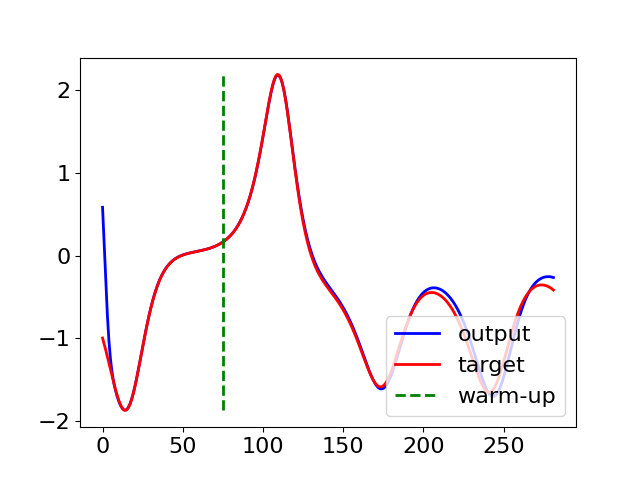
\includegraphics[width=\textwidth]{../Results/Lorenz-63/Figures/RNN-lstm-RDIM_3-N_used_50000-NUM-LAY_1-SIZE-LAY_100-ACT_tanh-ISH_statefull-SL_8-PL_4-LR_0.0001-DKP_1.0-ZKP_1.0-HSPL_300-IPL_200-NL_1-WID_0/prediction_augmend_TEST_33278.png}
			\caption{Prediction of first dimension}
		\end{subfigure}
%		\begin{subfigure}[b]{0.45\textwidth}
%			\includegraphics[width=\textwidth]{../\SixtyThreePath/prediction_TEST_\SixtyThreePathIndexOne_error.png}
%			\caption{Error of first dimension}
%		\end{subfigure}
		\begin{subfigure}[b]{0.45\textwidth}
			\includegraphics[width=\textwidth]{../\SixtyThreePath/prediction_TEST_\SixtyThreePathIndexOne.png}
			\caption{Predictions of all dimensions}
		\end{subfigure}
%		\begin{subfigure}[b]{0.5\textwidth}
		\begin{subfigure}[b]{\textwidth}
			\includegraphics[width=\textwidth]{../\SixtyThreePath/prediction_TEST_\SixtyThreePathIndexOne_contour.png}
			\caption{Contour plot}
		\end{subfigure}
		\caption{Test results for random initial condition \SixtyThreePathIndexOne}
		\label{63:predictions1}
	\end{figure}
	
	\begin{figure}[h]
		\centering
		\begin{subfigure}[b]{0.45\textwidth}
			\includegraphics[width=\textwidth]{../\SixtyThreePath/prediction_augmend_TEST_\SixtyThreePathIndexTwo.png}
			\caption{Prediction of first dimension}
		\end{subfigure}
%		\begin{subfigure}[b]{0.45\textwidth}
%			\includegraphics[width=\textwidth]{../\SixtyThreePath/prediction_TEST_\SixtyThreePathIndexTwo_error.png}
%			\caption{Error of first dimension}
%		\end{subfigure}
		\begin{subfigure}[b]{0.45\textwidth}
			\includegraphics[width=\textwidth]{../\SixtyThreePath/prediction_TEST_\SixtyThreePathIndexTwo.png}
			\caption{Predictions of all dimensions}
		\end{subfigure}
%		\begin{subfigure}[b]{0.45\textwidth}
		\begin{subfigure}[b]{\textwidth}
			\includegraphics[width=\textwidth]{../\SixtyThreePath/prediction_TEST_\SixtyThreePathIndexTwo_contour.png}
			\caption{Contour plot}
		\end{subfigure}
		\caption{Test results for random initial condition \SixtyThreePathIndexTwo}
		\label{63:predictions2}
	\end{figure}

	\FloatBarrier
\subsection{Lorenz-96}
	\newcommand{\NinetySixPath}{Results/Lorenz-96/Figures/RNN-lstm-RDIM_10-N_used_100000-NUM-LAY_3-SIZE-LAY_100-ACT_tanh-ISH_statefull-SL_8-PL_2-LR_0.0001-DKP_1.0-ZKP_1.0-HSPL_300-IPL_200-NL_1-WID_0}
	\newcommand{\NinetySixPathIndexOne}{25172}
	\newcommand{\NinetySixPathIndexTwo}{50168}
	
	\begin{figure}[h]
		\centering
		\begin{subfigure}[b]{0.45\textwidth}
			\includegraphics[width=\textwidth]{../\NinetySixPath/Loss_total_log.png}
			\caption{Training and validation loss}
			\label{96:loss}
		\end{subfigure}
		\begin{subfigure}[b]{0.45\textwidth}
			\includegraphics[width=\textwidth]{../\NinetySixPath/spectrum_comparison_TEST.png}
			\caption{Power spectrum for test predictions}
			\label{96:spectrum}
		\end{subfigure}
		\caption{Loss and power spectrum}
	\end{figure}

	Again \cref{96:loss} proves that the model learns and again no overfitting can be detected. However learning the Lorenz-96 proves to be significantly more difficult. This is to be expected, as this dataset is 10-dimensional, among other things. We therefore searched a lot for goot hyperparameters and also improved the learning rate scheduler, but the training always converged at a validation error of about 0.0011. The model's limited ability to predict the system is substantiated by the quality o the predictions of the test data. One can clearly see that only the first steps are correct but than prediction is off and evolves different. However, the Paper of Vlachas et alium, suggested that the LSTM should be able to fit to the Lorenz-96 system. This could be because we did not find the perfect hyperparameter. Futhermore, they used the stateless LSTM model while we used the statefull LSTM model. They also tried other models like the MSM or the combination MSM-LSTM. These models could eventually lead to better results. For the power spectrum we again use a smoothing factor $\sigma=50$ and a cutoff-frequency $f_{\text{cut}}=5000$. The spectra seems to fit well, but the differences are not clearly visible due to the peak at low frequencies.
	
	\begin{figure}[h]
		\centering
		\begin{subfigure}[b]{0.45\textwidth}
			\includegraphics[width=\textwidth]{../\NinetySixPath/prediction_augmend_TEST_\NinetySixPathIndexOne.png}
			\caption{Prediction of first dimension}
		\end{subfigure}
		\begin{subfigure}[b]{0.45\textwidth}
			\includegraphics[width=\textwidth]{../\NinetySixPath/prediction_TEST_\NinetySixPathIndexOne_error.png}
			\caption{Error of first dimension}
		\end{subfigure}
		%		\begin{subfigure}[b]{0.5\textwidth}
		\begin{subfigure}[b]{\textwidth}
			\includegraphics[width=\textwidth]{../\NinetySixPath/prediction_TEST_\NinetySixPathIndexOne_contour.png}
			\caption{Contour plot}
		\end{subfigure}
		\caption{Test results for random initial condition \NinetySixPathIndexOne}
		\label{96:predictions1}
	\end{figure}

	\begin{figure}[h]
		\centering
		\begin{subfigure}[b]{0.45\textwidth}
			\includegraphics[width=\textwidth]{../\NinetySixPath/prediction_augmend_TEST_\NinetySixPathIndexTwo.png}
			\caption{Prediction of first dimension}
		\end{subfigure}
		\begin{subfigure}[b]{0.45\textwidth}
			\includegraphics[width=\textwidth]{../\NinetySixPath/prediction_TEST_\NinetySixPathIndexTwo_error.png}
			\caption{Error of first dimension}
		\end{subfigure}
		\begin{subfigure}[b]{\textwidth}
			\includegraphics[width=\textwidth]{../\NinetySixPath/prediction_TEST_\NinetySixPathIndexTwo_contour.png}
			\caption{Contour plot}
		\end{subfigure}
		\caption{Test results for random initial condition \NinetySixPathIndexTwo}
		\label{96:predictions2}
	\end{figure}
	
	\FloatBarrier
	\printbibliography
\end{document}